\documentclass[./main.tex]{subfiles}

%\access{Advance Access Publication Date: Day Month Year}
%\appnotes{Original Paper}

\newcommand{\modafterreview}[1]{#1}

\begin{document}

%\subtitle{Sequence analysis}

\section{Graph analysis of fragmented long-read bacterial genome assemblies} \label{section:postassembly:knot}

Pierre Marijon, Rayan Chikhi, and Jean-St\'ephane Varr\'e\

\subsection{Abstract}
\textbf{Motivation:} Long-read genome assembly tools are expected to reconstruct bacterial genomes nearly perfectly, however they still produce fragmented assemblies in some cases. %Rather than proposing yet another assembler that performs incrementally better, it would be more informative to highlight why the existing ones fail on some  instances. 
It would be beneficial to understand whether these cases are intrinsically impossible to resolve, or if assemblers are at fault, implying that genomes could be refined or even finished with little to no additional experimental cost. \\
%
\textbf{Results:}  We propose a set of \modafterreview{computational} techniques to assist inspection of fragmented bacterial genome assemblies, through careful analysis of assembly graphs. %
By finding paths of overlapping raw reads between pairs of contigs, we recover potential short-range connections between contigs that were lost during the assembly process.  We show that our procedure recovers \modafterreview{45\% of missing contig adjacencies} in fragmented \canu assemblies, on samples from the NCTC bacterial sequencing project.
%The method consists of several components: extraction and visualization of intermediate graphs from assemblers, classification of contigs into chromosomal/plasmid origin, and retrieval of putative connections between contigs. \\
We also observe that a simple procedure based on enumerating weighted Hamiltonian cycles can suggest likely contig orderings. In our tests, the correct contig order is ranked first in half of the cases and within the top-3 predictions in \modafterreview{nearly all evaluated} cases, providing a direction for finishing fragmented long-read assemblies.\\

\textbf{Availability:} \url{https://gitlab.inria.fr/pmarijon/knot}\\

\subsection{Introduction}
Third-generation DNA sequencing using PacBio and Oxford Nanopore instruments is increasingly becoming a go-to technology for constructing reference genomes of non-model prokaryotes and eukaryotes. Longer sequencing reads allow in principle to overcome the reconstruction problems posed by genomic repetitions~\citep{tse}. Direct assembly of second-generation (Illumina) sequencing data typically also results in \modafterreview{high consensus accuracy} yet generally more fragmented bacterial assemblies~\citep{spades}. 
The large-scale ongoing NCTC project aims to assemble and make publicly available 3,000 bacterial strains sequenced using PacBio\footnote{https://www.sanger.ac.uk/resources/downloads/bacteria/nctc/}.


Recent works have demonstrated single-contig long-read assemblies of bacterial chromosomes~\citep{1chr1contig,loman2015complete}. 
Therefore, it is natural to ask whether genome assembly is now a solved problem with long reads\footnote{See e.g. \url{https://huit.re/PJMMA_uF}}, at minimum for smaller genomes such as bacteria. It turns out that in several cases, bacterial assemblies remain fragmented into a handful of contigs, even with long-read sequencing and recent assembly techniques. 
Deciding whether an assembly instance is resolved is not always clear due to the presence of plasmids, contaminants and unplaced low-quality reads. In this work, an assembly is considered to be \emph{resolved} if the number of contigs classified as chromosomal is equal to the expected number of chromosomes (generally \modafterreview{just} one, in the bacterial case).

 To date, the NCTC project contains 1,735 samples for which 1,136 have been assembled by the consortium, and among these, 599 (34\%) are unresolved according to the criteria above (as in Feb 2019). Later in this article, we will see that even when using multiple recent tools, many assemblies remain fragmented. Therefore there is a clear and unmet need for an investigation that determines whether those samples are intrinsically impossible to resolve, or whether current assembly methods are imperfect.

In this article we have selected a subset of NCTC samples (see Results section) and considered the outputs of three recent assemblers: \canu, \miniasm, and \hinge.
We observe that
instances where the assembly is fragmented can be challenging to further \modafterreview{manually} elucidate. 
In general, assemblers produce an assembly graph where nodes are contigs and edges reflect local sequence proximity in the genome (\emph{adjacency}). In fragmented instances, the final assembly graph is sometimes uninformative due to the absence of edges between contigs, hindering further assembly finishing steps. In such cases, it would be tempting to conclude that the assembly is fragmented due to regions of insufficient sequencing coverage, with no way to determine a likely contig order. However, in a number of cases we found that a lack of connectivity can be due to reads that were discarded early in the assembly pipeline. Here we will show that contig adjacency information can be computationally recovered from the raw data.
 
To automatically investigate unresolved assemblies and propose directions for refinement, we introduce a set of \modafterreview{\emph{in silico}} forensics operations for long-read assemblies, and we built a software framework. 
Our analyses are based solely on information present in the raw sequencing data \modafterreview{in addition to the contigs produced by a given assembly tool,} and are not biased by any other source, e.g. a closely related reference genome. For validation purposes \modafterreview{only} and to explain some of our observations, we will align contigs to a ground truth reference when one is available.
Our framework is first tested on synthetic data to illustrate a simple case of fragmentation due to heuristics in the \canu assembler.
We then show 
on real data
that our method helps recover useful adjacency information between contigs. 

Going further, we demonstrate how to use this recovered information to provide likely assembly hypotheses \modafterreview{using Hamiltonian paths}, through a ranked list of contigs orderings. Obtaining a small set of possible orderings between contigs, knowing that the true genome order is likely one of them, can be instrumental to guide further genome finishing steps.

\subsection{Related works}

Assembly forensics date back to the Sanger era, e.g. with the AMOSvalidate software~\citep{amosvalidate}, which detects mis-assemblies within contigs using multiple sources of information (e.g. read coverage, properly mapped pairs, clipping). Other tools have been introduced for mis-assembly detection in Illumina data (REAPR~\citep{REAPR}, FRCbam~\citep{FRCbam}, Pilon~\citep{Pilon}) and for PacBio data (VALET~\citep{VALET}) using similar principles. Completeness of an assembly can be estimated without any reference, using core genes as a proxy metric, e.g. with BUSCO~\citep{busco} or CheckM~\citep{parks2015checkm} software. Finally, assembly likelihood metrics have been introduced to assess the fit of an assembly to a probabilistic model of sequencing, via re-mapping reads to the assembly~\citep{clark2013ale,rahman2013cgal,ghodsi2013novo}.
For a more complete exposition, refer to a recent survey on metagenomics assembly validation~\citep{olson2017metagenomic}, that also largely applies to isolates.

For bacterial genomes specifically, several pipelines for \emph{assembly finishing} have been developed~\citep{bosi2015medusa}. They usually take as input an assembly obtained with short-read data and align it to one or multiple close reference genomes, in order to find a contig ordering~\citep{kremer2017approaches}.
Recent work has examined the cause of assembly fragmentation for seven bacterial genomes sequenced using PacBio sequencing, and rejected the hypothesis that gaps were caused by strong secondary DNA structure~\citep{utturkar2017case}. Instead, low coverage and repetitions appear to be the two main factors for contig termination.


To the best of our knowledge, little work has been carried to investigate assemblies based on the graph of assembled contigs or the initial string graph. Noteworthy exceptions are the Bandage software (an assembly graph visualization tool) ~\citep{bandage}, and the \hinge assembler that implements automated \modafterreview
{repeat handling based on the assembly graph}~\citep{hinge}. We use Bandage extensively in the present work, and \modafterreview{will consider datasets where even \hinge failed to produce a single-contig assembly}.

\subsubsection{Long-read assemblers}

Several genome assemblers have been developed to process third-generation sequencing data, either stand-alone ~\citep{canu,miniasm,hinge, abruijn} or in combination with Illumina data~\citep{dbg2olc,hybridspades,unicycler, zimin2013masurca}. 
In this work we will focus on three recent stand-alone assemblers, chosen because of their widespread usage (\canu), automated graph analysis algorithms (\hinge), and speed/modularity (\miniasm). However the  techniques are likely to be applicable to a broader set of assemblers.

\subsubsection{Description of \canu, \miniasm, and \hinge}

The \canu~\citep{canu} assembler consists of three major steps: correction, trimming and contig creation. The first two steps should not be regarded as innocuous pre-processing steps, as they significantly impact the rest of the assembly process.
%
The correction step uses MHAP to perform all-against-all read mapping then generates consensus reads with the falcon\_sense tool~\citep{falconsense}. \canu then performs overlapping of error-corrected reads with a legacy algorithm from the Celera assembler, named \textit{ovl}.
%
The trimming step detects hairpins, chimeric reads, and low-support regions and subsequently cuts reads.
%
A 'unitigging' step is performed using \texttt{bogart}, a modified version of CABOG~\citep{cabog}, to produce a graph that records only the longest overlaps between corrected reads (termed BOG for 'Best Overlap Graph'). 
\canu generates contigs from this graph 
and improves their consensus accuracy by re-mapping all reads.

The \miniasm pipeline consists of two separate tools: \minimap and \miniasm~\citep{miniasm}. \minimap finds overlaps between raw reads and outputs alignments.
\miniasm trims low-coverage regions of reads, then constructs a string graph from \minimap alignments that are suffix-prefix overlaps.
\miniasm performs simplification on the graph inspired by short-read assembly: transitive reduction, tip removal, bubble popping, and short overlaps removal based on a relative length threshold. 
After simplifications, non-branching paths are returned as contigs.

The \hinge~\citep{hinge} assembler uses raw uncorrected reads (similarly to  \miniasm) to construct an overlap graph similar to the BOG of \canu.
\hinge attempts to output finished bacterial assemblies through improved repeat-resolution. In cases where there subsist repetitions that are not spanned by reads, \hinge provides a visualization of the resulting assembly graph for manual inspection. 

\subsubsection{Assembly graphs}

Short-read and long-read assemblers output final assembly sequences in FASTA format, and an increasing number of tools also output an assembly graph in Graphical Fragment Assembly (GFA) format\footnote{\small\url{https://github.com/GFA-spec/GFA-spec}}. A final long-read \textbf{assembly graph} typically consists of all contig sequences as nodes, and a set of overlaps between contigs as edges. Assembly graphs 

Most long-read assemblers \modafterreview{start by constructing then analyzing} a \emph{string graph} (\textbf{SG}) of the reads~\citep{myers2005fragment}, where each read is a node, and overlaps between reads are represented by edges to which additional information is attached (e.g. overlap length, overlap error rate). In addition, transitive reduction is performed on the edges and reads \modafterreview{that are fully contained in others} are discarded.

\subsection{Methods}

We hypothesized that the final contig graph produced by assemblers does not always reflect all the information present in the raw data, and may be missing overlaps or \modafterreview{even} genomic regions.
We built a novel \modafterreview{algorithmic} framework to recover some of the 'missing' information and further analyze it. The main steps are presented in Fig.~\ref{fg:framework_presentation}, and the next sections describe them in more details. 


\begin{figure}[!tpb]
    \centering
    %\documentclass[a4paper]{article}
%
%\usepackage{tikz}
%
%\begin{document}


{\small
  \usetikzlibrary{arrows}
  \usetikzlibrary{shapes}
  \usetikzlibrary{positioning}
  \usetikzlibrary{calc}
  \usetikzlibrary{fit}
  
\tikzset{
    between/.style args={#1 and #2}{
         at = ($(#1)!0.5!(#2)$)
    }
}  
\begin{tikzpicture}

    \begin{scope}[node distance=0.5cm and 0.1cm]
        \node[draw,rounded corners=0.1cm] (0,0) (ac) {Assembly contigs};
        \node[draw,rounded corners=0.1cm, right=of ac] (rr) {Raw reads};

        \node[draw,rounded corners=0.1cm, below=of ac.west] (cc) {Contig classification};
        \node[draw,dotted,rounded corners=0.1cm, below=of rr.east] (isg) {Raw string graph};

        \node[between=cc and isg] (middle) {};
        \node[draw,dotted,rounded corners=0.1cm, below=of middle] (icps) {Inter-contigs paths search};

        \node[draw,dotted,rounded corners=0.1cm, below=of icps] (aag) {Augmented
          assembly graph};

        \node[draw,rounded corners=0.1cm, below=of aag] (pas) {Parsomonious assembly
        scenario};

      \draw[->] (ac) -- (cc);
      \draw[->] (rr) -- (isg);
      \draw[->] (cc) -- (icps);
      \draw[->] (isg) -- (icps);
      \draw[->] (icps) -- (aag);
      \draw[->] (aag) -- (pas);

      \node[draw,fit=(ac) (rr)] (r1) {};
      \node[draw,fit=(aag) (pas)] (r2) {};
  \end{scope}

    \begin{scope}[node distance=0em and 0em]
      \node[above=of r1.north,distance=0.01cm] {Input};
      \node[below=of r2.south,distance=0.01cm] {Output};
  \end{scope}

  
    \end{tikzpicture}
  }

%\end{document}

  
%%% Local Variables:
%%% mode: latex
%%% TeX-master: t
%%% End:

    \caption{The proposed framework takes as input raw long-read sequencing data and the output of an assembler. The \modafterreview{(optional)} contig classification step removes non-chromosomal contigs. A string graph of raw reads is constructed, in which paths are searched between extremities of contigs, then are converted into links between contigs in an augmented assembly graph. When such a graph is connected, putative contig orderings are reported. \modafterreview{Dotted nodes represent elements that are automatically visualized in the HTML report.}}
    \label{fg:framework_presentation}
\end{figure}

\subsubsection{Raw string graph}

First, we eliminate chimeric reads from the raw data based on overlaps found by \minimap using a custom tool\footnote{\small \url{https://gitlab.inria.fr/pmarijon/yacrd}} (manuscript in preparation~\citep{yacrd}, see Supplemental Fig. \ref{fig:appendix:yacrd}).
%because these chimeras create shortcuts and make paths falsely credible.
\modafterreview{
A string graph (SG) is then constructed using overlaps between \modafterreview{chimera-removed} reads \modafterreview{(here, overlaps found by \minimap)}.%, considering only the subset of reads not fully mapping inside contigs, i.e. just reads mapping to contig extremities (see Supplemental Section \ref{sec:appendix:read_filtering}).
} %found by \canu (\canu SG) and the other using those found by \minimap (\minimap SG). 
A stand-alone script was created to convert overlaps from the PAF format (defined in~\cite{miniasm}) to a graph in the GFA format\footnote{\small \url{https://gitlab.inria.fr/pmarijon/fpa}}. 
Transitive reduction over the edges of this SG is performed using Myers' algorithm~\citep{myers2005fragment}.

\subsubsection{Contigs classification \label{sub:classif}}

\modafterreview{
In order to simplify analyses and focus on chromosomal contigs, we filter out contigs of plasmid origin and contigs of unknown taxonomic status (see Supplemental Methods \ref{sec:appendix_contig_classification}). Contigs that were not marked as chromosomal are discarded. Note however that this contig classification step can be skipped in order to perform analysis of complete, unfiltered sets of contigs.}

\subsubsection{Computation of paths between contigs\label{sec:path_analysis}}

\modafterreview{An essential algorithmic component of our framework is the search for paths in the SG that uncover new connections between contigs.}
First, one read per contig extremity is identified \modafterreview{among reads included in the SG: a read is selected such that both its incoming and outgoing neighbors also map at the same contig extremity (in order to avoid selecting dead-end nodes in the SG).}  %(see details in Supplemental Section~\ref{sec:appendix_read_selection}). 

Then for each pair of contigs, shortest paths between reads at both extremities of each contig are computed in the SG \modafterreview{using Dijkstra's algorithm}.
\modafterreview{The length of a path is computed in nucleotides as follows: the sum of all reads lengths involved in the path minus all the overlaps between reads, as well as minus the overlaps between reads and contig extremities.}
\modafterreview{If contigs overlap, the path length is reported as zero.}
\modafterreview{Since we perform path search starting from each contig extremity}, we may obtain two shortest paths for each pair of contigs, and only the shortest of those two is kept. 
 
 %\pim{Je propose de supprimé le paragraphe suivant, il est devenue inutile}
 %In the rest of this article, we will mix-and-match contigs and SGs from different assemblers for the purpose of comparing assembly graphs. Typically, contigs will be taken from \canu, and SGs from \minimap and \canu, as \canu tends to produce longer contigs and \minimap produces a string graph with minimal use of heuristics.

\subsubsection{Augmented assembly graph \label{sec:aag}}

We transform a contig graph into a novel object, the \emph{augmented assembly graph} (\textbf{AAG}), as follows. Nodes of the AAG are contig extremities. An edge is inserted between two nodes if a path has been found by the procedure in Section~\ref{sec:path_analysis} between the two contig extremities. Each edge is weighted by the corresponding path length. Additionally, zero-weight edges are created between both extremities of each contig. 

Such a graph allows to explore adjacencies between contigs, \modafterreview{beyond those present in the original contig graph, in order to formulate hypotheses regarding the ordering of contigs}. \modafterreview{At a certain contig extremity, and in absence of genomic repeats, low-weight edges likely reflect adjacent contigs, while high-weight edges likely correspond to SG paths that pass through other contig(s) (i.e. transitively redundant edges in the AAG). In the presence of repeats, low-weight edges do not necessarily show true adjacencies between contigs, as the true path may be longer. %But it remains possible to filter out some edges.  % Rayan: pas compris comment
Yet one can observe that a path longer than the longest repeat in the genome necessarily reveals a distant link between two contigs (i.e. necessarily contigs which are truly non-adjacent on the genome), and also such path may go through another contig.}
%If a repeat exists at contig extremities the path should be shorter than the longest repeat.  % Rayan: pas nécessairement?}

\modafterreview{According to \cite{Treangen2009} most repetitions in bacteria are shorter than 10kbp.} 
We thus categorize edges \modafterreview{of the AAG} into 3 groups \modafterreview{according to their weight}.
Consider the path in the SG that led to the creation of the edge $e$ in the AAG between extremities of two different contigs $a$ and $b$.
If the path is longer than \modafterreview{10kbp}, and/or it contains at least one read that was involved in the construction of another contig $c$, the edge $e$ is named \emph{distant}. Otherwise the edge $e$ is considered to reflect an adjacency between $a$ and $b$. If there is more than one edge outgoing from the extremity of $a$ or of $b$, the edge $e$ is named a \emph{multiple adjacency} \modafterreview{(likely revealing a putative repeat)}. Otherwise it is named a \emph{single adjacency}.

\subsubsection{Searching for parsimonious assembly scenarios \label{sec:hamiltonian}}

% Why
We sought to determine whether contigs could possibly be ordered directly using the AAG. 
In principle, we anticipate to recover a large number of distant edges in the AAG, %\pim{la formule c'est n*(n-2)/2 ou n est le nombre d'extrémité mais on y est pas toujours}
therefore it would be non-trivial to determine a contig order by direct inspection of the graph layout (e.g. see Fig~\ref{fg:NCTC12123}). 
Given a connected AAG, our working hypothesis is that a minimum-weight Hamiltonian cycle may correspond to the correct contig order \modafterreview{(note that having a connected AAG is a necessary condition for such a cycle to exist, but not a sufficient one)}. This is guided by the intuition %truly adjacent contigs are more likely to be connected by short paths. 
that edges in the AAG with high weight are more likely to correspond to false connections due to repetitions or true paths between distant contigs.
For simplicity, we search for Hamiltonian cycles and not paths, under the assumption that the genome is circular. We further require that any Hamiltonian cycle traverses all zero-weight edges corresponding to both extremities of each contig. \modafterreview{Moreover, contigs mapping inside another one are not considered.} 

We designed an automated procedure to test this hypothesis, based on computing and sorting Hamiltonian cycles according to their total edge weights. %The weight of the Hamiltonian roads is based on the length of path we found between the ends of contig.
% Contig filter
In practice some of the AAGs that we obtain are too complex, due to the presence of short contigs (see the Discussion section for more details). \modafterreview{Our pipeline} %We therefore 
excluded contigs shorter than 100kbp from the \modafterreview{AAG} before listing all Hamiltonian cycles. 
%\pim{ceci est fais par knot directement désormais}
% Truth
For validation purposes, when a reference genome is available, we mapped all chromosomal contigs against this reference to determine the true contig order. We then recovered the position of the true \modafterreview{contig} order within the list of %contigs 
orders given by Hamiltonian cycles.

\subsubsection{Assembly report generation}

We implemented a Snakemake~\citep{snakemake} pipeline that takes as input \modafterreview{raw reads, contigs produced by an assembler, and optionally a contig graph. The pipeline follows steps described Fig.\ref{fg:framework_presentation}}, then generates an HTML report for easy inspection.
\modafterreview{Companion tools to compute AAG edge classification and to perform Hamiltonian path search are also provided.}

\subsection{Results}

\begin{figure*}[!htbp]
\centering
\subfloat[] {
\includegraphics[width=.3\textwidth]{paper/knot/img/t_roseus_canu_contigs.png}
\label{fg:t_roseus_contigs}
}
\subfloat[] {
 \includegraphics[width=0.35\textwidth]{paper/knot/img/t_roseus_projection.pdf}
 \label{fg:t_roseus_projection}
}
\subfloat[] {
 \includegraphics[width=0.22\textwidth]{paper/knot/img/t_roseus_dotplot.png}
 \label{fg:t_roseus_dotplot}
}

\modafterreview{
\subfloat[] {
	{\small
    \ttfamily
    
\begin{tikzpicture}
        \draw (0,0) node (1Left) {};
        \draw (8,0) node (1Right) {};

        \draw (8.3,0) node (8Left) {};
        \draw (10,0) node (8Right) {};

        \draw (10.3,0) node (4Left) {};
        \draw (15,0) node (4Right) {};
        
        % dessin des contigs
        \draw[fill] (1Left) ++ (0,0.1) rectangle node[above] {tig1} (1Right);
        \draw[fill] (8Left) ++ (0,0.1) rectangle node[above] {tig8} (8Right);
        \draw[fill] (4Left) ++ (0,0.1) rectangle node[above] {tig4} (4Right);
        
        % liens minimap qui respectent la reference NCTC
        \draw (1Right)
        .. controls +(up:5mm) and +(up:5mm) ..
        node[above] {491922} (8Left);
        
        \draw (8Right)
        .. controls +(up:5mm) and +(up:5mm) ..
        node[above] {ovl} (4Left);
        
        \draw[dotted] (1Right)
        .. controls +(up:12mm) and +(up:12mm) ..
        node[above] {755235} (4Left);
    
        % dessin du génome (en dernier pour masquer)
        \draw (0,0) -- (15,0);
    \end{tikzpicture}
}
   \label{fg:t_roseus_reconstruction}
}}

\caption{ 
Graph analysis of a synthetic dataset (\textsl{T. roseus}).
%
(a) Contig graph produced by \canu (visualized using Bandage): 3 contigs, no edge. 
%
(b) SG built from \minimap overlaps, on which  connected components of the \canu BOG are colored. 
% 
(c) Dot-plot of the \textsl{T. roseus} genome (NC\_018014.1) aligned against itself, showing a long tandem repeat.
%
(d) The AAG with \canu contigs ordered according to their position on the \textsl{T. roseus} reference. If two contigs overlap, no length is given and instead the link is labeled ’ovl’.
%Top (resp. bottom) edges between contigs reflect the length of a shortest path in the \canu SG (resp. \minimap SG).
}
\end{figure*}

\subsubsection{Datasets}

In order to illustrate our methods using a simple yet non-trivial case of assembly graph analysis, we simulated long reads from a linearized reference genome of \textsl{Terriglobulus roseus} (NC\_018014.1, 5.2 Mbp). \modafterreview{This genome contains an unusual 460kbp repeat that is challenging for assembly tools.} We used LongISLND \citep{longislnd}, with 20x sequencing coverage and 9kbp mean read length % , resulting in 11592 reads 
(Supplemental Table \ref{tb:appendix:t_roseus_20x}). 

To investigate real datasets, we mined the NCTC project which consists of 1735 bacterial strains (as of Feb 2019) sequenced using PacBio technology. For each dataset, the NCTC consortium had built an assembly using HGAP and Circlator~\citep{circlator} followed by a manual correction step.
%In the following we focus on \canu assemblies but the same work can be  obviously done on \miniasm assemblies.
We estimate, based on visual inspection of 159 NCTC fragmented \hinge assemblies\footnote{\url{https://web.stanford.edu/~gkamath/NCTC/report.html}} out of 997, that assembly graphs are missing contig adjacency information in 69\% of the fragmented assemblies of \hinge and \miniasm, i.e. around 13\% of all NCTC datasets \modafterreview{(including those that assemble perfectly)}.
Among datasets for which both \canu and \hinge failed to produce a single contig per chromosome, %and \canu contig graph contained more than one connected component \rc{on faisait ce test du nombre de composantes canu? ou alors 'canu' est une typo et c'était ma selection visuelle quand miniasm graph avait plusieurs components}\pim{comptage de contig},
we selected 19 datasets where the assembly made by NCTC contains as many chromosomal contigs as the number of expected chromosomes (i.e. is resolved), 24 datasets where the NCTC assembly is unresolved, and finally 2 datasets that were not yet assembled by NCTC.  See Supplemental Table \ref{tb:appendix:assembly_resume} for a complete list of the 45 datasets. 
All datasets were assembled with \canu version 1.7 and \miniasm version 0.2.

% Sur les 997 jeux de données de https://web.stanford.edu/~gkamath/NCTC/report.html, j'ai compté 159 jeux de données où hinge a marqué 'fragmented', et parmis ceux la, visuellement il y en à peu pres 110 où le graphe miniasm a plusieurs composantes connexes. si on compte ceux où il y a une seule composante minimap mais des dead-ends, ca fait environ 120 mais c'est surement sous-estimé (car minimap peut ne pas rapporter certains contigs)

\canu contigs were classified according to Section~\ref{sub:classif}. On average for each dataset, 10.2\% (resp. 6.4\%) of the \canu (resp. \miniasm) contigs are marked as plasmid, 13.7\% (resp. 12.2\%) do not match any bacteria in the Blast database and are therefore marked as of undefined origin, and the remaining 76.0\% (resp. 81.3\%) of contigs are classified as chromosomal and are further considered for analysis. Full classification results are presented in Supplemental Table \ref{tb:appendix:canu_NCTC_contigs} and \ref{tb:appendix:miniasm_NCTC_contigs}.

\modafterreview{We further investigated whether the assemblies %gaps at same locus or not in order to test whether or not we have 
   % 'complementary' assemblies that
   could somehow be combined, e.g. by improving \canu assemblies using \miniasm contigs. We have performed a simple test to evaluate this possibility (see Supplemental section \ref{sec:appendix:gap_comparison}) and could not straightforwardly improve assemblies this way.}

\subsubsection{Assembly graph analysis of a synthetic low-coverage dataset}

This section gives an introductory overview of the analyses that our method performs on the \textsl{T.roseus} simple synthetic dataset described above.
\canu produced 3 contigs of total length 4.7 Mbp. A $\approx$500kbp region is missing from the assembly. 
\miniasm produced 7 contigs and the \hinge assembler (commit 8613194) was not able to produce an assembly, likely because of the low coverage (20x).
%

% observations sur les graphes
Since the SG has a single connected component
(Fig.~\ref{fg:t_roseus_projection}) but both the BOG and the contig graph of \canu have multiple connected components (Fig.~\ref{fg:t_roseus_contigs}), assembly fragmentation can be explained by reads that have been discarded at the BOG construction stage of \canu.
%
The coloring of the SG using the connected components of \canu BOG (Fig.~\ref{fg:t_roseus_projection}) further suggests an ordering of contigs. Note that the \canu contig graph is uninformative on this dataset, as it contains no edges between contigs. 

% path analysis
We performed path analysis as per Section~\ref{sec:path_analysis}.
Fig.~\ref{fg:t_roseus_reconstruction} shows the length of paths in SG found between reads at \canu contigs extremities. Since a reference genome is available, the true order of contigs is reported on the Figure but note that path analysis does not need this information.
%
We find that the \canu contigs named tig8 and tig4 \modafterreview{overlap in the SG}. 
%
tig1 and tig8 are linked by a long path involving \modafterreview{491922bp}. This long path can be explained by looking at how tig1 has been built by \canu: the path goes through a large \modafterreview{'loop'} (see Supplemental Fig.~\ref{fg:appendix:t_roseus_tig1}) which corresponds to a repeat in the reference (Fig.~\ref{fg:t_roseus_dotplot}). The repeat (of length 460kbp) was not resolved by \canu, leading to a region of about 440kbp missing from the assembly between tig1 and tig8, which explains why the shortest path between both contigs contains as many as \modafterreview{491922bp}. 
We further checked that the path of length \modafterreview{755235bp} between tig1 and tig4 indeed contains reads from tig8, and is therefore redundant.
By aligning raw reads and \canu corrected reads to the reference genome, we observe a drop of raw reads coverage (around 8x) in the region between tig8 and tig4. This likely explains why \canu failed to connect both contigs.

As a side note, a \canu assembly of the same dataset with twice higher read coverage (40x) yielded a two-contig assembly, also with same pattern as in between tig8 and tig4. An older version of \canu (1.6) fully resolved the 40x dataset into a single contig, likely due to changes in how reads are corrected and trimmed between version 1.6 and 1.7.

\subsubsection{Investigation of 45 unresolved NCTC assemblies}

We performed the same type of analysis on the 45 NCTC samples. A \minimap AAG was constructed for each dataset using SG and \canu contig extremities. Assembly and AAG statistics are presented in Table \ref{tab:file_assembly_and_path_search_resume} for an excerpt of the dataset. 
\begin{table*}[htbp]
    \centering
    \scriptsize
    \modafterreview{
    \begin{tabular}{l|ccc|ccc|c|cc|ccc}
    \hline
     & \multicolumn{3}{c|}{NCTC contigs} & \multicolumn{3}{c|}{\canu contigs} &
     {\# nodes} &
     \multicolumn{2}{c|}{\# dead-ends in} & \multicolumn{3}{c}{\# edges in AAG} \\
     & & & & & &  & & & & & single & multiple \\
    NCTC ID & chr & pls & und & chr & pls & und & in AAG & contig graph & AAG & total & adjacency & adjacency
    \\\hline
    NCTC10006 & 1 & 0 & 0 & 3  & 0 & 0 &    4  & 2  & 2 & 4  & 2 & 0 \\
    NCTC10332 & 1 & 0 & 0 & 12 & 0 & 0 &    8  & 8  & 4 & 24 & 0 & 3 \\
    NCTC10444 & 1 & 0 & 0 & 7  & 0 & 0 &    8  & 3  & 0 & 24 & 0 & 6 \\
    NCTC10702 & 1 & 1 & 1 & 3  & 3 & 0 &    4  & 4  & 4 & 4 & 0 & 0 \\
    NCTC12123 & 2 & 3 & 0 & 5  & 4 & 1 &    6  & 4  & 1 & 12 & 1 & 2 \\
    NCTC12132 & 1 & 0 & 0 & 2  & 0 & 2 &    4  & 4  & 2 & 4  & 1 & 0 \\
    NCTC13125 & 1 & 2 & 4 & 6  & 3 & 1 &    6  & 0  & 0 & 12 & 0 & 4 \\
    NCTC13463 & 1 & 1 & 4 & 5  & 2 & 2 &    4  & 0  & 0 & 3  & 2 & 0 \\
    NCTC5050  & 2 & 3 & 0 & 4  & 2 & 3 &    6  & 6  & 0 & 12 & 3 & 0 \\
    \hline
    \end{tabular}
    }
    \caption{Assemblies and contig graphs statistics for an excerpt of 9 NCTC datasets (full tables in Supplemental Table~\ref{tb:appendix:assembly_resume} and \ref{tb:appendix:path_search_result}), consisting of 8 datasets where Hamiltonian cycle search succeeded, and the NCTC5050 dataset discussed in the Results section. AAGs are constructed using a SG built from \minimap overlaps and \canu contig extremities.  The 'contig graph' column corresponds to the final assembly graph produced by \canu; 'chr': number of chromosomal contigs; 'pld': number of plasmid contigs; 'und': number of other contigs. Note that some of \canu\xspace 'chr' contigs may be contained in others, therefore the '\# nodes in AAG' column corresponds to twice the number of non-contained contigs.}
    \label{tab:file_assembly_and_path_search_resume}
\end{table*}
Full statistics and more details are given in Supplemental Tables ~\ref{tb:appendix:assembly_resume}, \ref{tb:appendix:canu_NCTC_contigs} and \ref{tb:appendix:miniasm_NCTC_contigs}. 
There we observe that the number of contigs in \canu and \miniasm    assemblies is generally higher than in the assemblies made by NCTC.
%
Nevertheless the sum of lengths of chromosomal contigs is about the same in all assemblies (Supplemental Table \ref{tb:appendix:genomic_lengths}).

%Across the 45 datasets, the expected number of chromosomes is found only 4 times in terms of number of \miniasm contigs, three times with \hinge, and never with \canu. In some cases, \canu or \miniasm produce a large chromosomal contig of roughly the expected size, along with a few short contigs. % enlevé car on dit deja que ces 45 jeux de données sont fragmentés par canu et hinge

%\suppr{Contrarily to the simple \textsl{T. roseus} example, SGs of those imperfectly assembled NCTC datasets are not straightforward to visually inspect, which highlights the need to use automated tools.}

\paragraph{Case study of two NCTC datasets}

We closely examine two NCTC datasets that contain interesting patterns, through the lens of a ground truth obtained by remapping \canu contigs against respective NCTC assemblies using BWA-mem \citep{bwamem}.
%
%NCTC12123 is one of the \canu assemblies with the lowest number of chromosomal contigs (5), almost fully covering the NCTC assembly.
%NCTC5050 is a dataset for which the number of edges in the AAG is high relative to the number of \canu contigs. 
% 



\paragraph{NCTC12123} 

% firstly, we describe how the dataset was assembled by canu, miniasm and hinge
This dataset was assembled into 5 chromosomal  contigs by \canu, including 2 contigs that are contained in others and are automatically discarded by our pipeline (see Fig.~\ref{fg:NCTC12123}). 
\begin{figure*}[htbp]
    \centering
    \modafterreview{
	{\small
    \ttfamily
    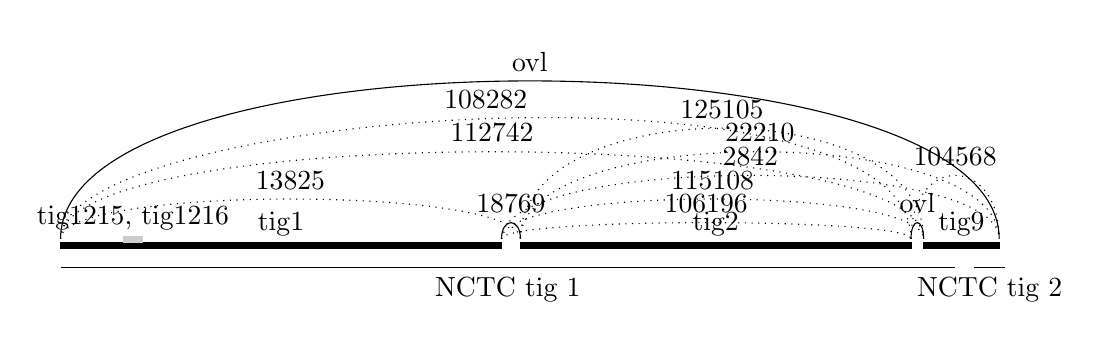
\begin{tikzpicture}[scale=0.8]
        \draw (0,0) node (1Left) {};
        \draw (7,0) node (1Right) {};
        
        \draw (7.3, 0) node (2Left) {};
        \draw (13.5, 0) node (2Right) {};
        
        \draw (13.7, 0) node (9Left) {};
        \draw (14.9, 0) node (9Right) {};
        
        \draw (1, 0.1) node (1215Left) {};
        \draw (1.3, 0.1) node (1215Right) {};
        
        % dessin des contigs
        \draw[fill] (1Left) ++ (0,0.1) rectangle node[above] {tig1} (1Right);
        \draw[fill] (2Left) ++ (0,0.1) rectangle node[above] {tig2} (2Right);
        \draw[fill] (9Left) ++ (0,0.1) rectangle node[above] {tig9} (9Right);
                
        % dessing des containments
        \draw[fill,color=black!20] (1215Left) ++ (0, 0.1) rectangle node[above,color=black] {tig1215, tig1216} (1215Right);
        
        % liens canu qui respectent la reference NCTC
        \draw (1Left)
        .. controls +(up:35mm) and +(up:35mm) ..
        node[above] {ovl} (9Right);
        
        \draw (1Right)
        .. controls +(up:5mm) and +(up:5mm) ..
        node[above] {18769} (2Left);
        
        \draw (2Right)
        .. controls +(up:5mm) and +(up:5mm) ..
        node[above] {ovl} (9Left);
        
        % liens canu qui ne respectent pas la reference NCTC
        \draw[dotted] (1Left)
        .. controls +(up:22mm) and +(up:32mm) ..
        node[above] {108282} (2Right);

		\draw[dotted] (1Left)
        .. controls +(up:10mm) and +(up:10mm) ..
        node[above] {13825} (2Left);
        
        \draw[dotted] (1Right)
        .. controls +(up:15mm) and +(up:15mm) ..
        node[above] {2842} (9Right);
       
         \draw[dotted] (1Right)
        .. controls +(up:5mm) and +(up:5mm) ..
        node[above] {106196} (2Right);

		\draw[dotted] (1Right)
        .. controls +(up:10mm) and +(up:10mm) ..
        node[above] {115108} (9Left);
        
        \draw[dotted] (2Left)
        .. controls +(up:20mm) and +(up:20mm) ..
        node[above] {22210} (9Right);
        
        \draw[dotted] (2Left)
        .. controls +(up:25mm) and +(up:25mm) ..
        node[above] {125105} (9Left);
        
        \draw[dotted] (2Right)
        .. controls +(up:15mm) and +(up:15mm) ..
        node[above] {104568} (9Right);
        
        \draw[dotted] (1Left)
        .. controls +(up:20mm) and +(up:20mm) ..
        node[above] {112742} (9Left);

        % dessin du génome (en dernier pour masquer)
        \draw (0,-0.3) -- node[below] {NCTC tig 1} (14.2,-0.3);
        \draw (14.5,-0.3) -- node[below] {NCTC tig 2} (15,-0.3);   
    \end{tikzpicture}} 
    }
    \caption{Mapping of \canu contigs (bold horizontal lines) against NCTC12123 assembly (the two thin horizontal lines). \modafterreview{Links between contigs give the length (in bp) of the shortest path in SG between reads at extremities. If two contigs overlap, no length is given and instead the link is labeled with 'ovl'}. 
    Plain links are paths that are compatible with the sequential order of contigs given  by mapping to the NCTC assembly, and dotted links are all other paths.}
    \label{fg:NCTC12123}
\end{figure*}

The assembly is made of 2 large contigs (tig1 and tig2) and a shorter one (tig9) totaling 4.78 Mbp. \miniasm produces also 5 chromosomal contigs, including 3 small ones. Both \canu and \miniasm contig graphs are made of two components. \hinge produces a single-component assembly graph but does not resolve it (because it detects multiple possible traversals). \modafterreview{Finally, the NCTC assembly consists of 2 chromosomal contigs: one being 4.69Mbp long and the other 21kbp long. Contigs tig1 and tig2 both map over the large NCTC contig, while tig9 maps to both NCTC contigs.}
%
%\jsv{quelle est la nature de ce segment de 21kpb,j'ai l'impression que le début map sur la fin et la fin sur le début du grand contig, i.e. il aurait pu permettre une circularisation}\pim{Ce fragment est semble t'il génomique (les contigs qui map dessus sont génomique) y compris le contig 9}
% resultat de yass de fasta_record_2 sur fasta_record_1
%fasta_record_2_selected_feature:_fasta_record_loc=4709233..4731063;/note="unitig_10|quiver|quiver";/label=chrom2;/colour=11_21831_bp	fasta_record_1	99.20	10174	68	13	11668	21831	2002718	1992548	0	1.41e+04
%fasta_record_2_selected_feature:_fasta_record_loc=4709233..4731063;/note="unitig_10|quiver|quiver";/label=chrom2;/colour=11_21831_bp	fasta_record_1	99.62	6788	2	24	15059	21831	1	6779	0	9.46e+03
%fasta_record_2_selected_feature:_fasta_record_loc=4709233..4731063;/note="unitig_10|quiver|quiver";/label=chrom2;/colour=11_21831_bp	fasta_record_1	100.00	4859	0	0	1	4859	4704374	4709232	0	6.98e+03
%
% secondly, what we bring
Using the AAG on \canu contigs (see Fig.~\ref{fg:NCTC12123}), one can observe that a number of scaffolding scenarios could be made following this graph. Interestingly, based on the mapping of the 3 contigs on the larger contig of the NCTC assembly, edges of smaller weight (i.e. shortest paths) tend to be associated with true contig adjacencies. In this example, low-weight Hamiltonian cycles (Section~\ref{sec:hamiltonian}) yield two likely contig orders (see Supplemental Fig.~\ref{fg:appendix:NCTC12123_solutions}).
%
% conclusion
This SG analysis thus enabled to retrieve an adjacency that was missed by \canu. It also confirms the multiple traversals prediction of \hinge, further reducing the number of putative contig orders to only two. 

% In the augmented assembly graph, we observe that edges of weight higher than 100 reflect that contigs are not adjacent. Both augmented assembly graphs built using \canu SG and \minimap SG are connected even when such edges are removed. Hamiltonian cycle search didn't result in an unique minimum-weight solution.  In Fig.~{\ref{fg:hamilton_path}}, two minimum-weight paths are found for this dataset (NCTC1213) with identical sums of weights: 1 -> 2 -> 9 and 1 -> 9 -> 2. Upon further inspection, this is due to an identical repetition between tig9/tig1 and tig1/tig2, see Fig~\ref{fg:appendix:dotplotNCTC12123} in the Appendix.


\paragraph{NCTC5050}

This dataset is assembled into 4 chromosomal contigs by \canu, including one that is contained in another. The \canu contig graph is 'fully' fragmented as each contig is its own connected component. There is no reference genome for this strain, and we chose as ground truth the NCTC assembly consisting of 2 contigs. One is entirely covered by a \canu contig, and the other contains the 3 remaining contigs (see Supplemental Fig.~\ref{fg:appendix:NCTC5050}). 
% DIT DANS LA FIH_GURE, INUTILE ICI In this figure, contigs are ordered according to their position on the two contigs of the NCTC assembly.
%
\modafterreview{
In the following, $x_s$ and $x_e$ denote left (resp. right) extremities of a contig $x$.
We found \emph{single} (i.e. non-repeat) adjacencies 
between tig1$_s$/tig23$_s$, 
tig1$_e$/tig10$_s$, 
tig10$_e$/tig23$_s$ that were confirmed by mapping to the longest contig from the NCTC assembly. Together, these single adjacencies suggest a putative scaffolding scenario: tig1 -- tig10 -- tig23(reversed). This scenario is also the top-ranked one proposed by our Hamiltonian path search procedure (see below).}

We also mapped corrected and raw reads to the junction for validation (see Supplemental Fig.~\ref{fig:appendix:NCTC5050_tig10_tig23}). We observe a drop of coverage at this location (see reads mapping in Supplemental Fig.~\ref{fig:appendix:NCTC5050_tig10_tig23}) that is likely the cause of assembly fragmentation. Therefore, again in this dataset the path search operation enabled to recover a link between contigs that was discarded by the assembler due to a drop in \modafterreview{sequencing} coverage.

% 
% enlevé cette partie hamiltonian vu qu'on a pas de vérité
%Similarly to NCTC12123, the number of possible paths could lead to a large number of putative contigs orders (see also Fig.~\ref{fg:contig_graph_NCTC5050}. Some paths could however be discarded because they go through another contig. For instance the path between extremity right of tig1 and extremity right of tig10 in \canu SG go through 23 reads of tig23. \pim{rajouté ces fichier de résultat en annexe ?}

\paragraph{Path search enables to recover adjacency between contigs}

\begin{table}[]
    \centering
    \small
    \modafterreview{
    \begin{tabular}{l c}
        Mean number of& \\
        \hline
         \canu contigs & 4.32 \\
         \hline
         Edges in AAG & 32.67 \\
         Theoretical max. edges in AAG & 41.83 \\
         Distant edges & 28.64 \\
         All adjacency edges & 4.02 \\
         Single adjacency edges & 1.16 \\
         Multiple adjacency edges & 2.86 \\
         \hline
         Dead-ends in \canu contigs &  4.94 \\
         Dead-ends in AAG, adjacency edges & 2.70 \\ % 1.2 en non repeat
        \hline
    \end{tabular}}
    \caption{Average statistics of augmented assembly graphs using a SG built from \minimap overlaps on \canu contigs across the \modafterreview{38} NCTC datasets \modafterreview{with two or more contigs, after size and classification filters}.
    All rows are as per definitions in Section~\ref{sec:aag}. 'Theoretical max. edges': number of possible edges in each AAG. 'Dead-ends in AAG, adjacency edges': number of dead-ends in the AAG when only adjacency edges are considered, i.e. distant edges are deleted.
    \label{tab:path_search_resume}}
\end{table}


Table~\ref{tab:file_assembly_and_path_search_resume} reports statistics of paths found between \canu contigs by our method for a subset of 9 NCTC datasets (for the full dataset, see Supplemental Table~\ref{tb:appendix:path_search_result}). 
%Our method detected between 3 and 7 adjacency edges in every dataset.
\modafterreview{We first focus on unambiguous contig adjacencies recovered by our pipeline.}
Single adjacency edges are only found in \modafterreview{6} out of 9 datasets, yet across the entire dataset of 45 samples, \modafterreview{60.4\%} of all single adjacency edges (\modafterreview{43} in total) are found in samples that have a sequencing coverage below 38x, and only \modafterreview{17} single adjacency edges are found in datasets with coverage above 38x. This is likely due to the error-correction step in assemblers that is less effective in low-coverage datasets (even when the true sequencing coverage is given to the assembler as a parameter), which in turn causes assembly fragmentation. Our method therefore enables to recover single adjacency edges between contigs that were fragmented due to this effect. 

To measure whether the \canu contig graphs could be used as-is to \modafterreview{recover contig order}, we counted the number of contig extremities that are not linked to any other extremity (i.e. \emph{dead-ends}). Those are contigs for which no chromosomal order can be reliably inferred.
In 35 out of the 45 datasets (7 out of 9 in Table~\ref{tab:file_assembly_and_path_search_resume}), the \canu contig graph has some dead-end extremities (between 1 and 23). In principle dead-ends extremities should not exist in circular bacterial assembly graphs, except for linear chromosomes. \modafterreview{Assemblers, here \miniasm and} \canu, do not report all \modafterreview{true} contig adjacencies. \modafterreview{In contrast}, our method enables to recover some of these adjacencies and lower the number of dead-ends in \modafterreview{23 out the 37} datasets (and all but one \modafterreview{dataset} in Table~\ref{tab:file_assembly_and_path_search_resume}).
% enlevé car potentiellement polémique
%, and in 4 datasets all dead-ends are 'elucidated', i.e. have a putative single or multiple adjacency in the AAG. 

% enleve pour gagner de la place
%In addition, NCTC5053 is an interesting case where none of the NCTC contigs are classified as chromosomal. Our analysis was able to recover single adjacency links between all 5 non-contained contigs.  \rc{6 contigs, 4 edges single adjacency AAG, il en manque un ou alors un contig est contenu.. (même si il y avait 32 edges total)} 

Table \ref{tab:path_search_resume} summarizes average AAG statistics over all \modafterreview{38} datasets on \canu contigs (per-dataset results in Supplemental Table~\ref{tb:appendix:path_search_result}). \modafterreview{Results for \miniasm contigs are shown in Supplementary Tables~\ref{tab:appendix:path_search_resume_miniasm} and~\ref{tb:appendix:path_search_result}.} On average, \canu contig graphs contain \modafterreview{4.32} nodes (\modafterreview{5.86} extremities), among which \modafterreview{4.94} extremities are dead-ends. The AAG enables to reduce the number of dead-end extremities to \modafterreview{2.7 (45\% lower)}, through the discovery of \modafterreview{1.16} single adjacency edges and \modafterreview{2.86} multiple adjacency edges in the AAG \modafterreview{per dataset on average}. \modafterreview{The reduction is also significant for \miniasm contigs but not as high (31\%, Supp. Table~\ref{tab:appendix:path_search_resume_miniasm}).} Note that these adjacencies are 'real' in the sense that they are all supported by paths \modafterreview{of overlapping reads} of \modafterreview{total nucleotide} length less than 10kbp, yet a number of them may be caused by repetitions. An upper bound on the ability to mine paths in the SG is given by the theoretical maximal number of edges in the AAG (\modafterreview{41.83} edges). Our method is \modafterreview{on average 78\%} close to this bound for \canu contigs \modafterreview{(resp. 90.1\% for \miniasm)} as it discovered \modafterreview{32.67} edges \modafterreview{per dataset (resp. 85.1)}. We note that large fraction (\modafterreview{87\%}) of \modafterreview{discovered edges} were classified as distant edges, yet the remaining adjacency edges are informative as they significantly contribute to removing dead-ends in the contig graph.

\paragraph{Contig order search retrieves parsimonious assembly scenarios}

While the work done in the previous section helps to recover contig adjacencies, the presence of multiple adjacency edges due to repetitions often prevents us from unambiguously inferring a contig order.
We applied the Hamiltonian cycle procedure presented in Section~\ref{sec:hamiltonian} to determine likely contig orderings. Fig.~\ref{fg:hamilton_path} shows orderings sorted by weight across \modafterreview{23} datasets on which the method could successfully be executed (connected AAG, low number of edges).
\begin{figure}[!tpb]
	\centerline{\includegraphics[scale=0.5]{paper/knot/img/hamilton_path.png}}
    \caption{Weights of scenarios in AAGs. Each curve correspond to the sorted list of Hamiltonian cycles, sorted by weight. If a ground truth is known, a diamond symbol marks the correct assembly scenario. Extended Figure available in Supplementary material \ref{fig:appendix:hamilton_path}}
    \label{fg:hamilton_path}
\end{figure}

A ground truth is known in only 8 of those datasets. Among them, the lowest-weight scenario is ranked first in \modafterreview{3 datasets, 2nd in 2 datasets, 3rd in 1, 4th in 1 and 38th in the last one}. 

These results suggest that the correct assembly scenario is likely to be one of the top predictions made by our parsimonious Hamiltonian cycle procedure. However finding many fragmented datasets that also have a ground truth is inherently difficult, thus further work is needed to confirm this hypothesis. Also, datasets where several scenarios have similar weights (i.e. curves that 'plateau' in Fig~\ref{fg:hamilton_path}) will possibly be more challenging to resolve using this method. \modafterreview{Yet} for many samples with fragmented assemblies, parsimonious assembly scenarios are a promising approach to explore a limited number of hypotheses that could further be validated using long-range PCR to finish the genome.

\subsection{Discussion}

We presented a set of concepts to provide novel insights on fragmented long-read bacterial genome assemblies. 

By searching for paths of overlapping raw reads between extremities of contigs, we construct an \textit{augmented assembly graph} that recovers unreported adjacencies between contigs. We demonstrate several usages of this graph: to provide a more informative representation of fragmented assemblies, to examine repeat structures, and to propose likely contig orderings. In our tests, the AAGs of NCTC datasets \modafterreview{recover edges for nearly half (45\%) of the dead-end nodes in \canu contig graphs, on average}. We further show a link between \modafterreview{the lowest}-weight Hamiltonian cycles in the AAG and the \modafterreview{true} contig order. We highlight that our method solely relies on the raw data and information produced by assemblers at various stages of their pipelines and, \modafterreview{when our contig classification step is skipped,} no reference genome nor external information (e.g. genome map, \modafterreview{BLAST database}) \modafterreview{are} used. 


%% Le SG est un overlap graph
Our method hinges on \modafterreview{directly} constructing a string graph on the raw reads, \modafterreview{after a relatively conservative chimera removal step}. Doing so avoid biases that may be introduced in the read trimming and error-correction steps \modafterreview{ of an assembler. Indeed, overlaps between reads may become shorter or even absent after error-correction}. For instance on the 45 NCTC datasets that we analyzed, the number of edges in SGs built from \canu error-corrected reads is reduced by 41.4\% compared to the SGs of raw reads.
%
%We used minimap because it was the fastest and the one that used the least memory while having a correct sensitivity and accuracy.~\citep{bench_ovl} % j'ai enleve car on considere aussi le canu SG
%
%We use \minimap for generate this graph because they are the best in computation time and memory usage and they have resanoable 
%
%We chose to consider an overlap graph over uncorrected reads (\minimap SG) as \minimap has high \pim{j'ai envie de mettre not to bad parceque minimap1 a quand même une sensibility de 59.6 sur jeux de donnée réel pacbio, mais c'est peut-être un peut aggrésif} overlap sensitivity, precision, and performance~\citep{bench_ovl}. 
%However uncorrected SGs include all raw reads regardless of their accuracy. As such, a \minimap SG may contain false information such as spurious overlaps.
%
% disriminé les jonctions les chemins différent que sur la longueur
We have classified edges in the AAG, by considering their \modafterreview{underlying nucleotide} lengths and whether \modafterreview{they contain} reads \modafterreview{that} belong to other contigs. %: a short path likely reflects genomic proximity, whereas long paths seem to be indicative of coverage gaps or connectivity through repetitions. 
To go further, one could define confidence metrics, e.g. based on local graph structures.

Due to a combination of engineering choices and the inherent difficulty of visualizing large assembly graphs, our software has only been tested on bacterial genomes and is unlikely to readily run on larger genomes. However, the techniques presented here (AAG, path search between contig extremities, weighted Hamiltonian cycles) are not specific to bacterial assembly, and should in principle be applicable to small and large eukaryotes. 
However more work would be needed e.g. to scale path search to thousands of contigs, refine thresholds (contig filter, adjacency edges), handle inter-chromosomal repeats, and \modafterreview{an evaluation of the relevance of Hamiltonian cycles for larger genomes}.

We stress that our techniques currently do not aim at detecting misassemblies within contigs. We also did not focus on the difficulty of running multiple assembly programs, but we note that the process has previously been reported to be challenging~\citep{Lariviere347625}. %Detecting misassemblies requires radically different methods%, such as the ones implemented in Tigmint ~\citep{jackman2018tigmint}.
Our work is also orthogonal to assembly reconciliation~\citep{alhakami2017comparative}, which consists of constructing a higher-contiguity assembly by merging the results of multiple assemblers.

%We sometimes observed that \canu and \miniasm fragmented assemblies at similar locations. % peu appuyé donc enlevé
No attempt was made to \modafterreview{optimize the detection of} overlaps between reads %,  or recover true overlaps between contigs that went unnoticed in assembly graphs, 
though \modafterreview{this could be} a direction for improvement. 
Finally, automatic post-assembly improvements based on the AAG would be a natural extension of this work. \modafterreview{One could use the AAG to design an oracle that suggests a limited number of (long-range) PCR experiments for resolving individual repeats.} 
% remarque d'antoine : de maniere generale insister plus sur le fait qu'on met en oeuvre quelque chose de simple qui permet dans XX\% des assemblages testés de les ameliorer}

%\pim{This study present useful framework to understand fragmentation assembly and help finishing assembly but it also confirms what HINGE has shown, that an in-depth study of the assembly graph could improve the quality of assemblies, and that more tools must be developed to analyze these graphs.} % insisté sur le finishing dans l'intro et l'abstract

\subsection*{Acknowledgements}

This work was supported by an Inria doctoral grant and the INCEPTION project (PIA/ANR‐16‐CONV‐0005). The authors are grateful to Samarth Rangavittal, Monika Cechova, Jason Chin, Jason Hill and Christopher W. Wheat for discussions that led to this project,  Gautam Kamath for guidance on reproducing NCTC analyses with \hinge, Antoine Limasset and anonymous reviewers for helpful comments on the manuscript.


\end{document}


